\documentclass[	11pt, ]{fphw}

\usepackage[utf8]{inputenc} 
\usepackage[T1]{fontenc}
\usepackage{mathpazo}\usepackage{graphicx} 
\usepackage{booktabs} 
\usepackage{listings} 
\usepackage{enumerate} 
\usepackage[english]{varioref}

\title{Assignment \#2} %
\author{Anita Mezzetti} 
\institute{École polytechnique fédérale de Lausanne} 
\class{Global Business Environment} 
\professor{Luisa Lambertini} 

%--------------------------------------------------------------------
\begin{document}
\maketitle 
\section*{Question a}
The authors refers to a first prospective, according to which the U.S. deficit can be interpreted in terms of trade flows and associated payments. In this case, the main reason of this deficit can be found into the patterns of U.S trades. This countries imports more goods and services than the ones that it exports. Therefore, households, firms and government must borrow the difference on international capital markets. The current account deficit reflects the fact that U.S payments greatly exceed the payments received by foreigners. This means that there is a big imbalance in U.S international trade.
However, Bernanke claims that these factors cannot explain the size of the current account imbalance or its recent sharp increase. Consequently, he suggests another viewpoint whereby the main reason of current account deficit is described in terms of investment and national saving. He emphasizes this prospective. Firstly, he remembers that economic growth requires many investments. In a closed economy, only the savings finance these expenditures and, in each period, the financial flows are balanced. However, this vision is unlikely: today all economies are open. This permits to a country to borrow the amount required to finance domestic investments from abroad. As a result, the financial flows are unbalanced: one country’s deficit equals the excess of its investments over its saving.


\section*{Question b}
Theoretically, the current account level of the world’s countries should sum zero. So, the increase in the U.S. current account deficit between 1996-2003 must be balanced by a shift toward surplus of equal magnitude in other countries. \\
According to Bernanke, the emergence of a global saving glut explains the change of International capital flows. One origin of the saving glut is the saving motivation of rich countries with aging citizens. Many progressive economies face an apparent lack of domestic investments, because of declining workforces and capital-labor ratios. The prospective of domestic returns is low; then many industrial countries try to create a current account surplus. 
However, this saving behaviour does not explain much. Instead, we have to focus on developing economies: they develop from being net users to finance international capital markets. Moreover, the current account of the other industrial countries declined between 1996 and 2003, causing a $\$$410 billion increase in the U.S. current account deficit. Only a small fraction was offset by an increased surplus in other industrial nations.


\section*{Question c}
One motivation can be found in the decline in the U.S. national saving rates. \\
The main reason that caused this change is the series of financial crises that affected developing countries. In the mid-1990s, these economies imported capital, but they did not use it in a productive way. This combined with other factors (as overestimated fixed exchange rates and debt) led to the crisis. Actually, the effects of this crisis brought many changes: these countries were obliged to find new strategies. From being net importers, they started to export.\\
We have to consider also the change in the demographic composition of developed countries: an higher number of retirees relative to the number of workers. This lead to an increase in the saving in industrialised countries. \\
Another factor is the sharp rise of oil prices. The Middle Est and some other countries run the oil market, so their current account surplus has risen.
%Also equity prices caused the capital flows changes from about 1996 to 2000. In fact, U.S. economy, with its technological development and rising productivity, was very attractive for international investors. There was a big capital flow toward U.S. 
%The dollar was strong and US consumers preferred to import, considering that exports were more expensive. This created, on terms of international flows, a rising imbalance.


\section*{Question d}
Yes, there is a relationship. Firstly, after the crisis of developing countries, they became net exporter nations. This strategy has pushed these economies toward current account surpluses. As inevitable consequence, the current account of industrial countries has decreased accordingly. \\
Moreover, these developing countries invested in US, an attractive destination during the technology boom.  This increased the amount of cashflows from developing countries in developed countries.\\
The growth of the current account of developing nations reflects their strategy, based big international outflows through the financial markets.
%In addition, dollar is the leading international reserve currency. So dollar-denominated assets have directed the saving emissions of emergent nations. 
therefore, events outside U.S. borders have influenced the evolution of its current account deficit.

\section*{Question e}
The United States economy was attractive for foreign investors  during the technology boom and the depth and sophistication of the country's financial markets have been important. So, the movement toward surplus in developing country current accounts has had a different impact on the United States relative to other industrial countries.\\
Another factor is the special international status of the U.S. dollar. The dollar was strong, so US consumers preferred to import, considering that exports were more expensive. This created, on terms of international flows, a rising imbalance. The developing world has headed its saving flowing out more to dollar-denominated asset.   \\
The effects of the saving outflow may thus have been felt disproportionately on U.S. interest rates and the dollar (considering the appreciation for cheaper imports).  \\

\par However, the United States were not an unique case. The current account deficit of some other developed countries, as France, Italy, Spain, Australia and U.K., has raised since 1996. While Germany and Japan increased their current account. 
This is because the last two nations have not increased household wealth and have not run into housing appreciation. 

\section*{Question f}
For basic economic logic, developed countries should lend on net to the developing countries in the long term and raise their current account surplus. In this way, industrial nations would produce higher returns, while the others would have the opportunity to invest to promote development and better living standards. In fact, most developing countries, contrary to developed ones, have younger and more-rapidly growing workforces, as well as relatively low ratios of capital to labor. These conditions imply that the returns to capital in those countries may potentially be quite high. 


\section*{Question g}
The author do not believe that the deficit would decrease only balancing the federal budget by itself. He also thinks that the deficit cannot be eliminate in the near future. 
He is certain that decreasing the federal budget deficit is a good idea, even if the effects would be modest. The principal effects might be increased consumption and a consequent decrease in saving rather than a lower current account deficit. \\
He also supports increasing household savings, even if the effects on U.S. deficit might not be dramatic. This can be done, for example, by creating tax-favoured saving vehicles in order to be independent from foreign investors. This policy would support productivity and would help to make better previsions.  \\
In addition, outward-looking policies should be applied, considering that some reasons of the deficit are external to U.S.. Developing countries should improve their investments and remove barriers to the free flow of financial capital; in order to restore their natural role as borrowers. Helping these countries could reduce the risk of other financial crises. Thus, it would increase both the willingness of those countries to accept capital inflows and the willingness of foreigners to invest there, and therefore reduce the Global Savings Glut. \\
All these solutions are likely to decrease U.S. current account deficit gradually. 


\section*{Question h} 

\begin{figure}[h]
\centering 
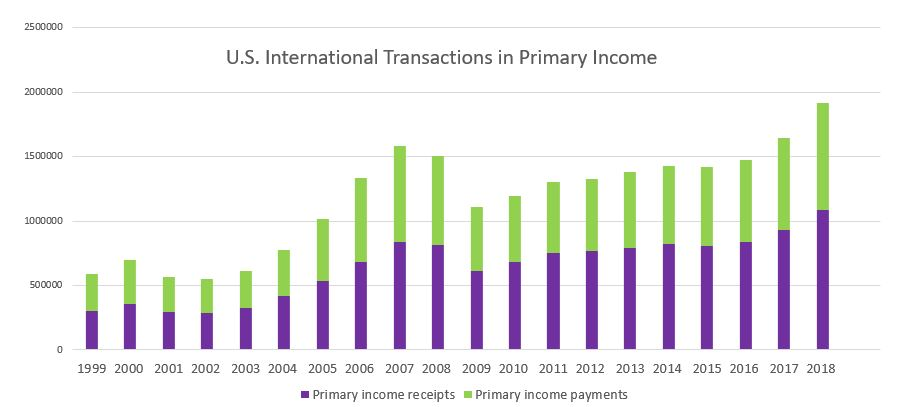
\includegraphics[scale=0.80]{ass2eshzero.JPG} 
\caption{Question h} 
\label{1}
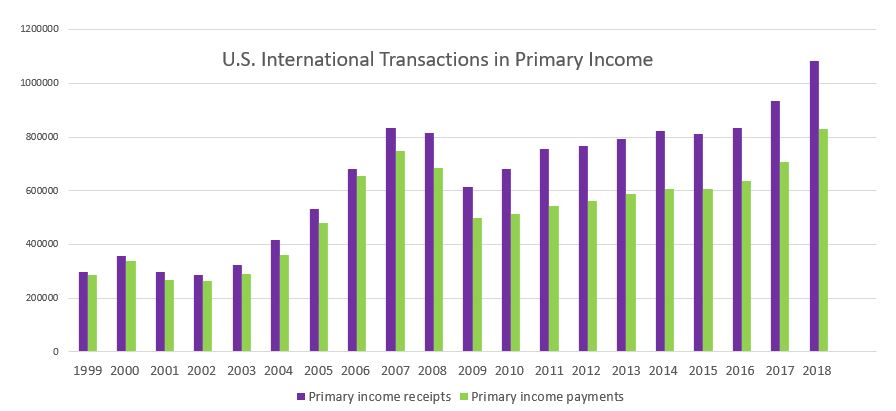
\includegraphics[scale=0.80]{ass2esh.JPG} 
\caption{Question h}
\label{2}
\end{figure}

The primary income account shows primary income flows between resident and nonresident institutional units. It is calculated as the difference between the income domestic residents earn on wealth they invested in other countries (primary income receipts) less the payments domestic residents make to foreign owners of wealth that is used in their country (primary income payments).
\par Looking the primary income trend (Figure \vref{1}), without differences between the payments and the receipts, we can see that the transactions levels rose at the beginning of the century. Then they drop in 2008, perhaps due to the global financial crisis. Then the cash flows started to grow; slowly between 2009 and 2016 and more quickly in the last years. 
\par The Figure \vref{2} points out a positive gap between the receipts and the payments. We can observe it from 1999 up to today, but it has started to grow in the second part of the 2000s. After the financial crisis, U.S. primary income receipts increased faster than the payments, boosting the gap. In fact the receipts returned to the before crisis values in a few years, while the payments took longer. 
It is important to remember that the developing countries, attracted by the dollar-strength, invest in U.S.. 


\section*{Question i}

\begin{figure}[h]
\centering 
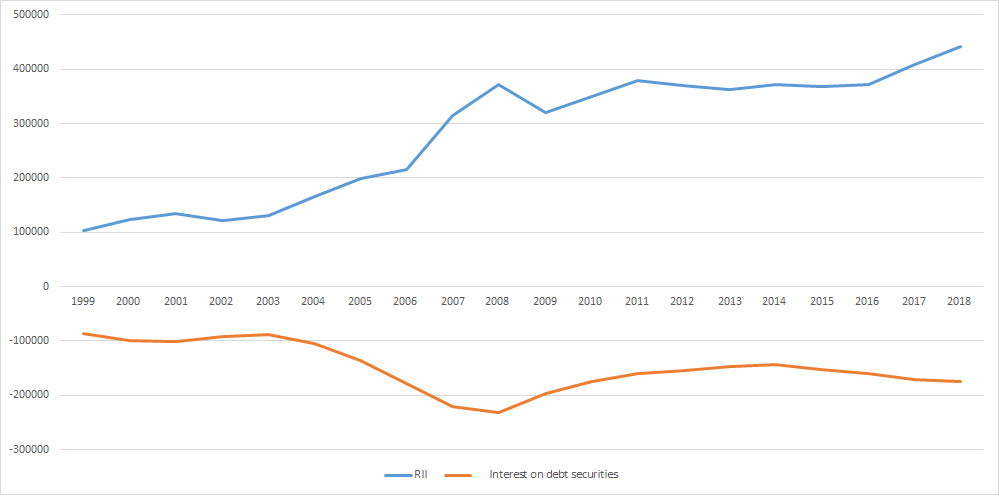
\includegraphics[scale=0.8]{ass2esi.png} 
\caption{Question i} 
\label{3}
\end{figure}
An investment income represents the money that someone earns from an increase in the value of investments. Risky Investment Income shows the amount of capital invested by residents in risky assets. \\
The Figure \vref{3} displays that RII is always positive. That means that U.S. is most disposed to invest in these risky assets than foreigners. This value increase quite quickly after 2002. In that period, there was a big technological development in U.S.  the financial crisis stopped this positive trend. However, the value decreased only for one year, then the RII grew again. From 2011 to 2016, the value remained almost stable and it has risen since 2016.
\par Regarding the other line, firstly it is evident that all values are negative. They represent the interest on debt securities. \\

Debt securities have an implicit level of safety and they are typically classified by their level of default risk: the lower is their risk,  the lower is the interest rate. The interest rate is largely determined by the perceived repayment ability of the borrower; higher risks of payment default usually lead to higher interest rates to borrow capital. \\
In the graph, there are represented net values, so we are always talking about the difference between receipts and payments. So, negative net interests on debt securities imply that interests on payments are higher than interests on receipts. Then foreign investors take less risk than U.S. (assuming that returns of U.S. securities  are not remarkably bigger). \\
The interest on debt securities decreased in 2008: in this period of crisis the difference between interest on payments and receipts grew (see Figure \vref{4}). This means that U.S. pays more interests than the interests received. 

\begin{figure}[h]
\centering 
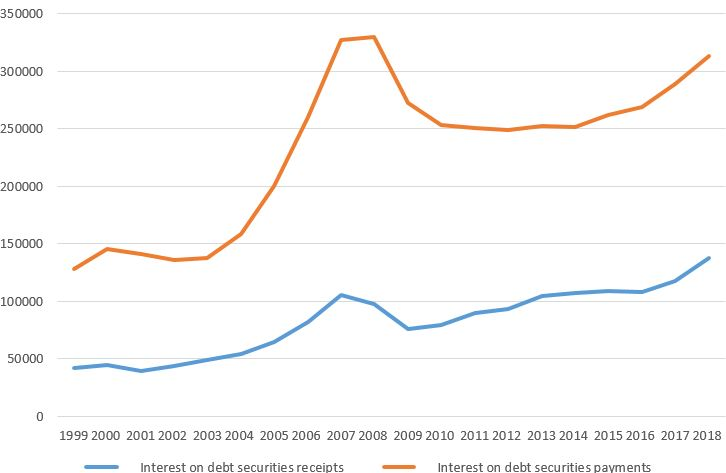
\includegraphics[scale=0.6]{ass2esi2.JPG} 
\caption{Question i} 
\label{4}
\end{figure}

\end{document}